% \section{Implementation Matters}\label{sect:appendix_implementation}


% To circumvent this complexity, TODOName avoids re-encoding those tokens. Instead, we manipulate existing token representations to make them reusable between LLM instances. Our approach is inspired by TODO RoPE scaling, H2O, Streaming LLM.



% TODO\begin{enumerate}
%     \item main setup: single GPU, single LLM, this has advantages
%     \item we store cache 'blocks' and stitch them together just in time, one layer at a time
%     \item block position and context can change over time. Normally, it would require re-encoding
%     \item instead, we simply rotate blocks to a new offset just-in-time - which can be done by multiplying them by a pre-determined cos/sin pair - and then concatenate them together - we call that RoPE stitching
%     \item RoPE stitching can potentially be fused into attention computation, but this is future work
%     \item also consider distributed setup, where sync frequency can be important
% \end{enumerate}

% % \begin{figure}[t]
% %     \centering
% %     
\includegraphics[width=\linewidth, height=150px]{resources/placeholder.png}
% %     \caption{(left) shared cache definition framework used in our reference implementation[TODOclickable] (right) compiling this cache for batched inference with RoPE stitching.}
% %     \label{fig:cache_manager_and_rope_stitching}
% % \end{figure}


% \section{Prompting Details}\label{sect:appendix_prompts}

% TODO HERE BE DRAGONS

% \section{Few-shot examples}\label{sect:appendix_examples}

% TODO HERE BE DRAGONS

\section{Examples}\label{sect:appendix_examples}

In this section, we present a reasoning chain, generated by Hogwild!\! Inference with an interleaved cache layout and token-wise synchronization.
We denote our intervention in model generation in \textit{italics} and highlight worker interactions with \textbf{bold} to enhance readability.
\subsection{Example from LIMO math dataset}\label{sect:appendix_example_1}
\textit{Problem:} For $t = 1, 2, 3, 4$ , define $S_t = \sum_{i = 1}^{350}a_i^t$ , where $a_i \in \{1,2,3,4\}$ . If $S_1 = 513$ and $S_4 = 4745$ , find the minimum possible value for $S_2$

\textit{> Bob [1]: Hi, I'm Bob.} Let me suggest that we first model this as an optimization problem with constraints. We have variables representing the number of each $a_i$ equal to $1,2,3,4$. Let me denote the counts as $n_1,n_2,n_3,n_4$ where $n_1 + n_2 +n_3 +n_4 =350$. Then $S_1=1 n_1 +2n_2 +3n_3 +4n_4 =513$. $S_4=1^4n_1 +2^4n_2 +3^4n_3 +4^4n_4 = n_1 +16n_2 +81n_3 +256n_4=4745$. We need to minimize $S_2= n_1 +4n_2 +9n_3 +16n_4$. So with variables $n_1,n_2,n_3,n_4$ non-negative integers. Since there are three equations and four variables, we can express variables in terms of some parameters and find the minimum $S_2$.

\textit{> Alice [1]: Hi, I'm Alice. Here's how we should do this:} Since we need to minimize $S_2$ given $S_1=513$ and $S_4=4745$, with each $a_i$ being $1,2,3,4$. Let me think of variables $n_1,n_2,n_3,n_4$ as the counts of each number. So $n_1 +n_2 +n_3 +n_4=350$. The first moment $S_1 =n_1 +2n_2 +3n_3 +4n_4=513$. The fourth moment $S_4 =n_1 +16n_2 +81n_3 +256n_4=4745$. We need to minimize $S_2 =n_1 +4n_2 +9n_3 +16n_4$. Let me write down the equations:

Equation 1: $n_1 +n_2 +n_3 +n_4=350$,

Equation 2: $n_1 +2n_2 +3n_3 +4n_4=513$,

Equation 4: $n_1 +16n_2 +81n_3 +256n_4=4745$.

% \textit{> Alice [2]:}  Equation 4: $n_1 +16n_2 +81n_3 +256n_4=4745$.

\textit{> Bob [2]:} \textit{Sanity check: am I doing redundant work? (y/n):} Let me see. \textbf{Alice is setting up the variables and equations. I can proceed to express variables in terms of others. Let me try to subtract equation 1 from equation 2} to get $(n_2 +2n_3 +3n_4)=513-350=163$. So Equation 2 - Equation 1 gives: $(n_2 +2n_3 +3n_4)=163$. Let me call this Equation A.

\textit{> Alice [3]:}  \textbf{Let me also subtract equation 1 from equation 4}: Equation 4 - Equation 1 gives $15n_2 +80n_3 +255n_4 =4745-350=4395$. Simplify this equation by dividing by $5$: $3n_2 +16n_3 +51n_4=879$. Let me call this Equation B.

\textit{...<Bob tried one approach and it did not gave results>...}
% \textit{> Bob [3]:} 1$5n_2 +80n_3 +255n_4 =4395$. Hmm, perhaps we can simplify further. Let me divide by common factors. $15n_2 +80n_3 +255n_4 =4395$. Let me see: $15$ is a common factor for first and third terms: $15(n_2 + 17n_4) +80n_3 =4395$. Hmm, not sure yet. Alternatively, maybe find another relation.

\textit{> Bob [4]:}  Let me note that Equation A: $n_2 =163 -2n_3 -3n_4$. Substitute this into Equation B: 
\textit{...<Bob did math simultaneously with Alice starting from Equation B to derive Equation C>...}
% $3\cdot (163 -2n_3 -3n_4) +16n_3 +51n_4 =879$. Let me compute this:

% $$3\cdot 163 = 489,$$
% $$3\cdot (-2n_3) = -6n_3,$$
% $$3\cdot (-3n_4) =-9n_4,$$
% Thus, equation becomes:

% $489 -6n_3 -9n_4 +16n_3 +51n_4 =879 \to 489 +10n_3 +42n_4 =879 \to 10n_3 +42n_4 = 390 $ divide by $2$ 
$5n_3 +21n_4=195$. \textbf{Same as Alice's Equation C}.

\textit{> Alice [4]:} \textit{Sanity check: am I doing redundant work? (y/n):} Let me see. \textbf{Bob is working on equation B. Let me see if we can express variables in terms of others.} Let me let variables be $n_1,n_2,n_3,n_4$. From Equation A: $n_2 +2n_3 +3n_4 =163$. \textit{...<Alice did math simultaneously with Bob starting from Equation A to derive Equation C>...}
% Let me solve for $n_2$: $n_2 =163 -2n_3 -3n_4$. Substitute this into Equation B: $3\cdot (163 -2n_3 -3n_4) +16n_3 +51n_4 =879$. Let me compute that: $489 -6n_3 -9n_4 +16n_3 +51n_4 =879 \to (489) + (10n_3 +42n_4)=879$. So 1$0n_3 +42n_4 = 879-489=390$.
Simplify this equation by dividing by common factors. Let me see $10$ and $42$ have GCD $2$: divide both sides by $2$: $5n_3 +21n_4=195$. Let me call this Equation C: $5n_3 +21n_4=195$.

\textit{> Bob [5]:} \textit{Sanity check: am I doing redundant work? (y/n):} Yes, \textbf{Alice is already working on equation C. Let me see what else I can do.} 
\textit{...<Bob tried different thing and it did not gave results>...}

% Let me try to express $n_3$ in terms of $n_4$ from equation C: $5n_3 =195 -21n_4 \implies  n_3=(195-21n_4)/5= 39 - (21/5)n_4$. Hmm, so $21n_4$ must be congruent to $195 \mod5$. Since $195 \mod5=0$, so $21n_4$ must be divisible by $5$. Since $21 \mod5=1$, so $n_4 \mod5$ must be $0$. So $n_4$ must be multiple of $5$. Let me let $n_4=5k$, where $k$ is integer $\geq0$. Then $n_3=39 -21\cdot (5k)/5=39-21k$. Wait, wait: $n_4=5k$. So substituting back:

% $$n_3= (195 -21\cdot (5k))/5 = (195 -105k)/5 = 39 -21k.$$

\textit{> Alice [5]:}  Equation C: $5n_3 +21n_4=195$. Let me see possible integer solutions. Let me write this as $5n_3 =195 -21n_4 \implies  n_3 = (195-21n_4)/5$. For $n_3$ to be integer, $195 -21n_4$ must be divisible by $5$. Let me compute $21n_4 \mod5. 21 \mod5=1$, so $21n_4 \mod5 =n_4 \mod5$. Thus, $195 \mod5=0$, so $195 -21n_4 =0 \mod5 \implies  -21n_4 =0 \mod5 \implies  -n_4 =0 \mod5 \implies  n_4 =0 \mod5$. \textbf{Therefore, $n_4$ must be a multiple of $5$.} Let me let $n_4=5k$, where $k$ is a non-negative integer. Then $n_3=(195 -21\cdot (5k))/5 = (195 -105k)/5 =39 -21k$. Since $n_3$ must be non-negative, $39-21k \geq0 \implies  21k \leq39 \implies  k \leq39/21 \approx 1.857$. So $k$ can be $0,1$. Because $k$ must be integer. \textit{...<Alice double checked herself>...}
% Wait, $39/21=1.857$ so $k$ can be $0$ or $1$. Wait, $21\cdot 1=21$, so $39-21=18$, which is positive. If $k=2$, then $39-42=-3 <0$. So $k$ can only be $0$ or $1$. Hmm, so possible $n_4$ is $0$ or $5$. Let me check:

If $k=0$: $n_4=0$, then $n_3=39-0=39$.

\textit{> Bob [6]:} \textit{Sanity check: am I doing redundant work? (y/n):} \textbf{Alice is working on expressing $n_3$ and $n_4$. Let me see if I can find other relations.} \textit{...<Bob tried to find similar equations with no result>...}
% Let me also note that $n_1 =350 -n_2 -n_3 -n_4$ from Equation 1. Since $n_2=163-2n_3-3n_4$ (from Equation A), substituting into $n_1$ gives: $n_1=350 - (163-2n_3-3n_4) -n_3 -n_4 =350-163 +2n_3 +3n_4 -n_3 -n_4=187 +n_3 +2n_4. So n_1=187 +n_3 +2n_4$. So all variables expressed in terms of $n_3$ and $n_4$. Since we have $n_4=5k$, and $n_3=39-21k$. Let me substitute into $n_1$:

% $$n_1=187 + (39-21k) +2\cdot (5k)=187+39-21k+10k=226 -11k.$$


\textit{> Bob [8]:} \textit{Sanity check: am I doing redundant work? (y/n):} \textbf{Alice is handling case1. Let me handle case2 when $k=1$.}

\textit{> Alice [6]:} \textit{Sanity check: am I doing redundant work? (y/n):} Let me proceed. So $n_4$ can be $0$ or $5$. Let me check both possibilities:

Case1: $k=0 \implies n_4=0, n_3=39$. 
\textit{...<Alice did math cheking case1 where $k=0$>...}
% Then $n_2=163-2\cdot 39 -3\cdot 0=163-78=85$. Then $n_1=187 +39 +0=226$. Let me check total variables: $226+85+39+0=350$ <correct>. Check $S_1$: $226\cdot 1 +85\cdot 2 +39\cdot 3 +0\cdot 4=226+170+117+0=513$ <correct>. Check $S_4$:$226 +16\cdot 85 +81\cdot 39 +256\cdot 0=226+1360+3159+0=4745$ <correct>.
So this case is valid.

% \textit{> Alice [7]:}  Wait, let's compute $S_2$ for each case. 

\textit{> Alice [8]:}  For Case1 ($k=0$):
$$S_2 = n_1 +4n_2 +9n_3 +16n_4 =226 +4\cdot 85 +9\cdot 39 +0 =226 +340 +351= 226+340=566;$$
$$ 566+351=917.$$

\textit{> Bob [9]:}  Let me check for $k=1$. \textit{...<Bob did math cheking case2 where $k=1$>...}
% So $n_4=5$, $n_3=39-21\cdot 1=18$. Then $n_2=163 -2\cdot 18 -3\cdot 5=163-36-15=112$. Then $n_1=187 +18 +2\cdot 5=187+18+10=215$. Check total:$215+112+18+5=350$ <correct>. $S_1$:$215 +224 +54 +20=513$ <correct>. $S_4$:$215 +16\cdot 112 +81\cdot 18 +256\cdot 5=215+1792+1458+1280=215+1792=2007; 2007+1458=3465; 3465+1280=4745$ <correct>. So case2 is valid. Now compute $S_2$ for case2: $S_2=215 +4\cdot 112 +9\cdot 18 +16\cdot 5$. $4\cdot 112=448$, $9\cdot 18=162$, $16\cdot 5=80$. Total:$215+448=663$; $663+162=825$; $825+80=905$.
So between the two cases, the minimum $S_2$ is $905$. 

\textit{> Alice [9]:} \textit{Sanity check: am I doing redundant work? (y/n):} \textbf{Bob is checking $k=1$.} Let me compute $S_2$ for both cases. 

\textit{...<Alice validated their approach>...}

\textit{> Bob [10]:} <Bob validated their approach> \textbf{earlier we deduced} $n_4$ must be multiple of $5$ because $n_4 =0 \mod5$. Because $21n_4 =n_4 \mod5$ must be $0$. So yes, only multiples of $5$. Thus only $k=0$ and1. So $905$ is the minimal. 

\textit{> Alice [11]:}  So the minimal $S_2$ is $905$. \textit{...<Alice once again checking answer>...}

\textit{...<Alice and Bob validated their solution checking corner cases>...}

\textit{> Alice [17]:} \textit{Sanity check: am I doing redundant work? (y/n):} Let me confirm with the earlier computations. For $k=1$, $S_2=905$, which matches. So yes. Thus the minimal is $905$. But the problem states that $a_i$ are in $\{1,2,3,4\}$, so the counts must be non-negative integers, which they are in both cases. So the minimal $S_2$ is $905$. Therefore, the answer is \boxed{905}.


\section{Additional LIMO evaluations}\label{sect:appendix_extra_plots}

Here, we report a more detailed breakdown of our evaluation on LIMO tasks from Section~\ref{sect:experiments}. Namely, we consider include additional budgets and arrange our results on a common plot.

\begin{figure}[h]
    \centering
    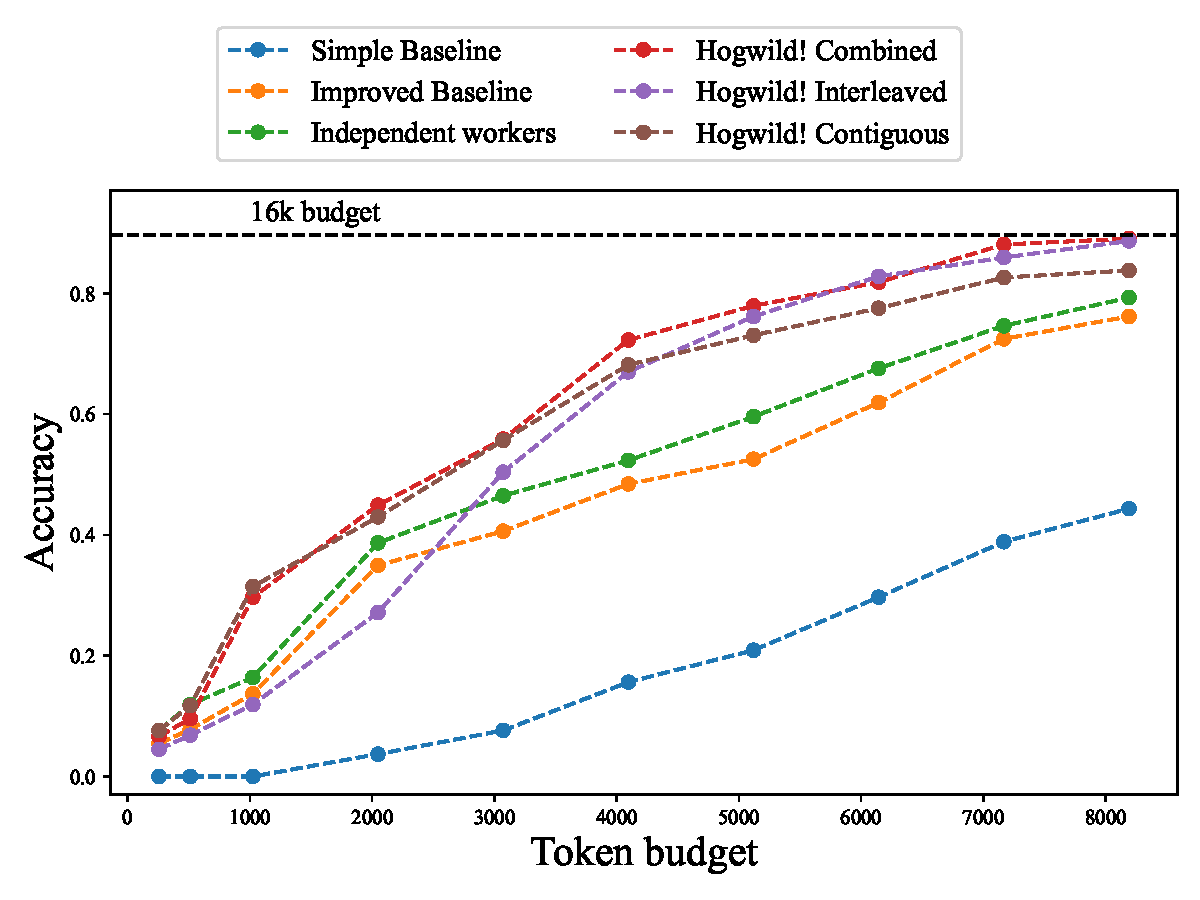
\includegraphics[width=\linewidth]{resources/method_comparison_limo.pdf}
    \caption{Detailed comparison of various parallel inference setups and baselines on LIMO task set, in the same setup as in Section~\ref{sect:experiments}.}
    \label{fig:limo_detailed_plot}
\end{figure}